\documentclass[pdftex,12pt,a4paper]{article}

\usepackage[slovak]{babel}
%\usepackage[IL2]{fontenc}
\usepackage[utf8]{inputenc}
\usepackage{fancyhdr}
\usepackage{mathtools}
\usepackage{hyperref}
\hypersetup{pdfborder={0 0 0}}
\usepackage[final]{pdfpages}
\usepackage{graphicx}
\usepackage{epstopdf}
\usepackage{subfigure}
\usepackage[top=3cm, bottom=3cm, right=2.5cm, left=2.5cm]{geometry}

\usepackage{listings}
\usepackage{color}
\usepackage{textcomp}
\definecolor{listinggray}{gray}{0.9}
\definecolor{lbcolor}{rgb}{0.95,0.95,0.95}
\lstset{
	backgroundcolor=\color{lbcolor},
	tabsize=4,
	rulecolor=,
	language=matlab,
        basicstyle=\scriptsize,
        upquote=true,
        aboveskip={0.3\baselineskip},
        columns=fixed,
        showstringspaces=false,
        extendedchars=true,
        breaklines=true,
        prebreak = \raisebox{0ex}[0ex][0ex]{\ensuremath{\hookleftarrow}},
        frame=single,
        showtabs=false,
        showspaces=false,
        showstringspaces=false,
        identifierstyle=\ttfamily,
        keywordstyle=\color[rgb]{0,0,1},
        commentstyle=\color[rgb]{0.133,0.545,0.133},
        stringstyle=\color[rgb]{0.627,0.126,0.941},
}

% matrix columns
\makeatletter
\renewcommand*\env@matrix[1][*\c@MaxMatrixCols c]{%
  \hskip -\arraycolsep
  \let\@ifnextchar\new@ifnextchar
  \array{#1}}
\makeatother

% norm command
\newcommand{\norm}[1]{\left|\left|#1\right|\right|}
% adj command
\newcommand{\adj}{\operatorname{adj}}
% rank command
\newcommand{\rank}{\operatorname{rank}}
% m command (matrix)
\newcommand{\m}[1]{\mathbf{#1}} 

\def \nazovUlohy{Uživatelská príručka pre automat na jízdenky}
\def \skola{\textbf{ČVUT FEL - Kybernetika a Robotika}}
\def \tema{Úloha z APO (Architektúra počítačov)}
\def \author{\textbf{Michal Šustr} \\ \textbf{Matúš Cvengroš}}
\def \date{21. 4. 2012}

\fancyhead[L]{\skola \\ \nazovUlohy} 
\fancyhead[R]{\author}
\fancyfoot[C]{\thepage}
\renewcommand{\headrulewidth}{0.4pt}
\renewcommand{\footrulewidth}{0.4pt}
\renewcommand{\refname}{\section{Zoznam použitej literatúry}}

\hypersetup{
    bookmarks=true,         % show bookmarks bar?
    unicode=false,          % non-Latin characters in Acrobat’s bookmarks
    pdftoolbar=true,        % show Acrobat’s toolbar?
    pdfmenubar=true,        % show Acrobat’s menu?
    pdffitwindow=false,     % window fit to page when opened
    pdfstartview={FitH},    % fits the width of the page to the window
    pdftitle=\nazovUlohy,    % title
    pdfauthor=\author,     % author
    pdfsubject=\tema,   % subject of the document
    pdfnewwindow=true,      % links in new window
    colorlinks=true,       % false: boxed links; true: colored links
    linkcolor=blue,          % color of internal links
    citecolor=green,        % color of links to bibliography
    filecolor=magenta,      % color of file links
    urlcolor=blue           % color of external links
}


\begin{document}
\begin{center}
	\makebox[4cm][l]{
\includegraphics[width=3cm]{/home/michal/.latex/lev.png}}
	\parbox[s][4cm][s]{10cm}{\scshape \large
	České vysoké učení technické v Praze\\Fakulta elektrotechnická\\Katedra kybernetiky}
	\vskip 2cm {\Huge \bfseries \nazovUlohy}
	\vskip 1cm {\Large \tema}
\end{center}

\vfill

\begin{flushright}
	\author \\
	~\\
	\date
\end{flushright}


\newpage
\pagestyle{fancy}

Najprv si zvolíme aké lístky si chceme kúpiť stlačením príslušných tlačidiel, na displeji je nápis \texttt{Zvolte jizdenky}
\begin{figure}[htb]
	\begin{center}
		\leavevmode
		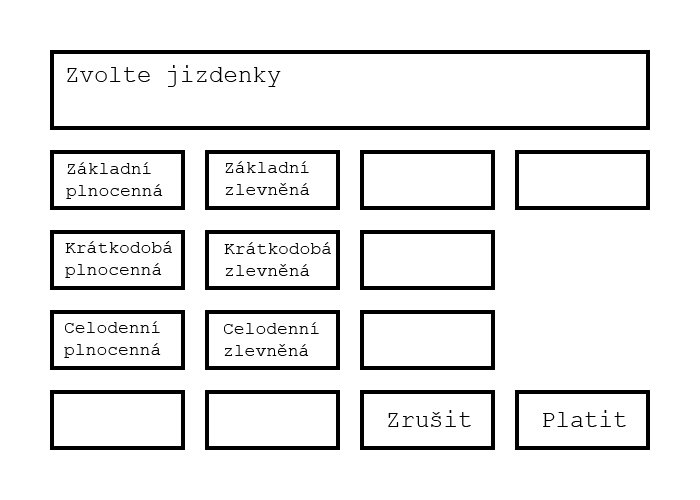
\includegraphics[width=0.6\textwidth]{zvolte-jizdenky.png}
	\end{center}
\end{figure}

Automat priebežne ukazuje, akú celkovú sumu budeme musieť za lístky zaplatiť. Keď už sme s výberom spokojní, prejdeme na platenie tlačidlom \texttt{Platit}
\begin{figure}[htb]
	\begin{center}
		\leavevmode
		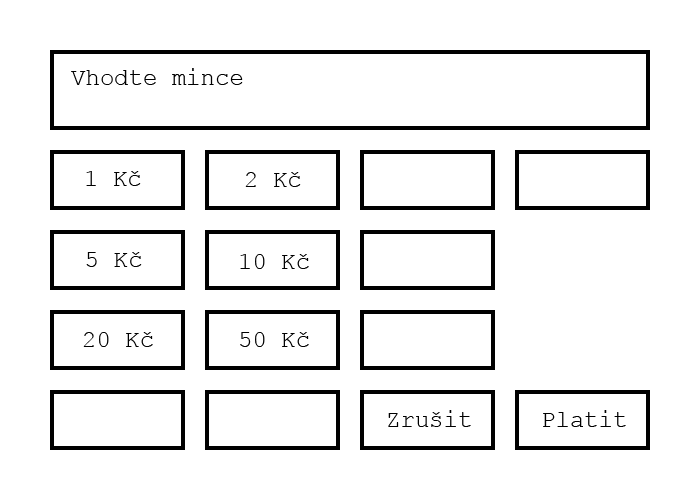
\includegraphics[width=0.6\textwidth]{vhodte-mince.png}
	\end{center}
\end{figure}

Vhadzovanie mincí simulujeme stláčaním príslušných tlačidiel, pričom automat ukazuje, akú čiastku je treba ešte vložiť. Keď vložíme presnú sumu, dostaneme naše lístky, a ak by bola suma vyššia, automat sa nám pokúsi vydať pokiaľ má nejaké mince.

V hocijakej fázi môžeme stlačiť tlačítko zrušiť, ktoré zruší objednávku a vráti nám mince, pokiaľ sme nejaké vložili.

\end{document}